%%%%%                                                                   %%%%%
%%%%% Remember to set the details for your submission in 0_setinfo.tex    %%%%%
%%%%%                                                                   %%%%%

\section{Introduction}    

The group work for this exercise has been really helpful.The exercise has also helped us to understand the importance of teamwork and communication in project management. We have learned how to work together effectively, delegate tasks, and communicate clearly.

\subsection{Background information}

The Chinese Fusion Engineering Test Reactor (CFETR) as shown in \cref{fig:CFETR} is a proposed tokamak designed to bridge the technical gap between ITER and a commercial demonstration power plant (DEMO). Planned for two-stage operation, the facility will initially target a fusion power output of 200 MW \parencite{CFETRCONFIG2022}. The second phase involves upgrading the machine to exceed 1 GW of fusion power. This stage aims to perform tokamak DEMO validation, to achieve a duty factor of 0.3-0.5 and to ensure tritium self-sufficiency with a Tritium Breeding Ratio (TBR) >1 \parencite{CFETRCONFIG2019}.

\begin{figure}[htbp]
\centering
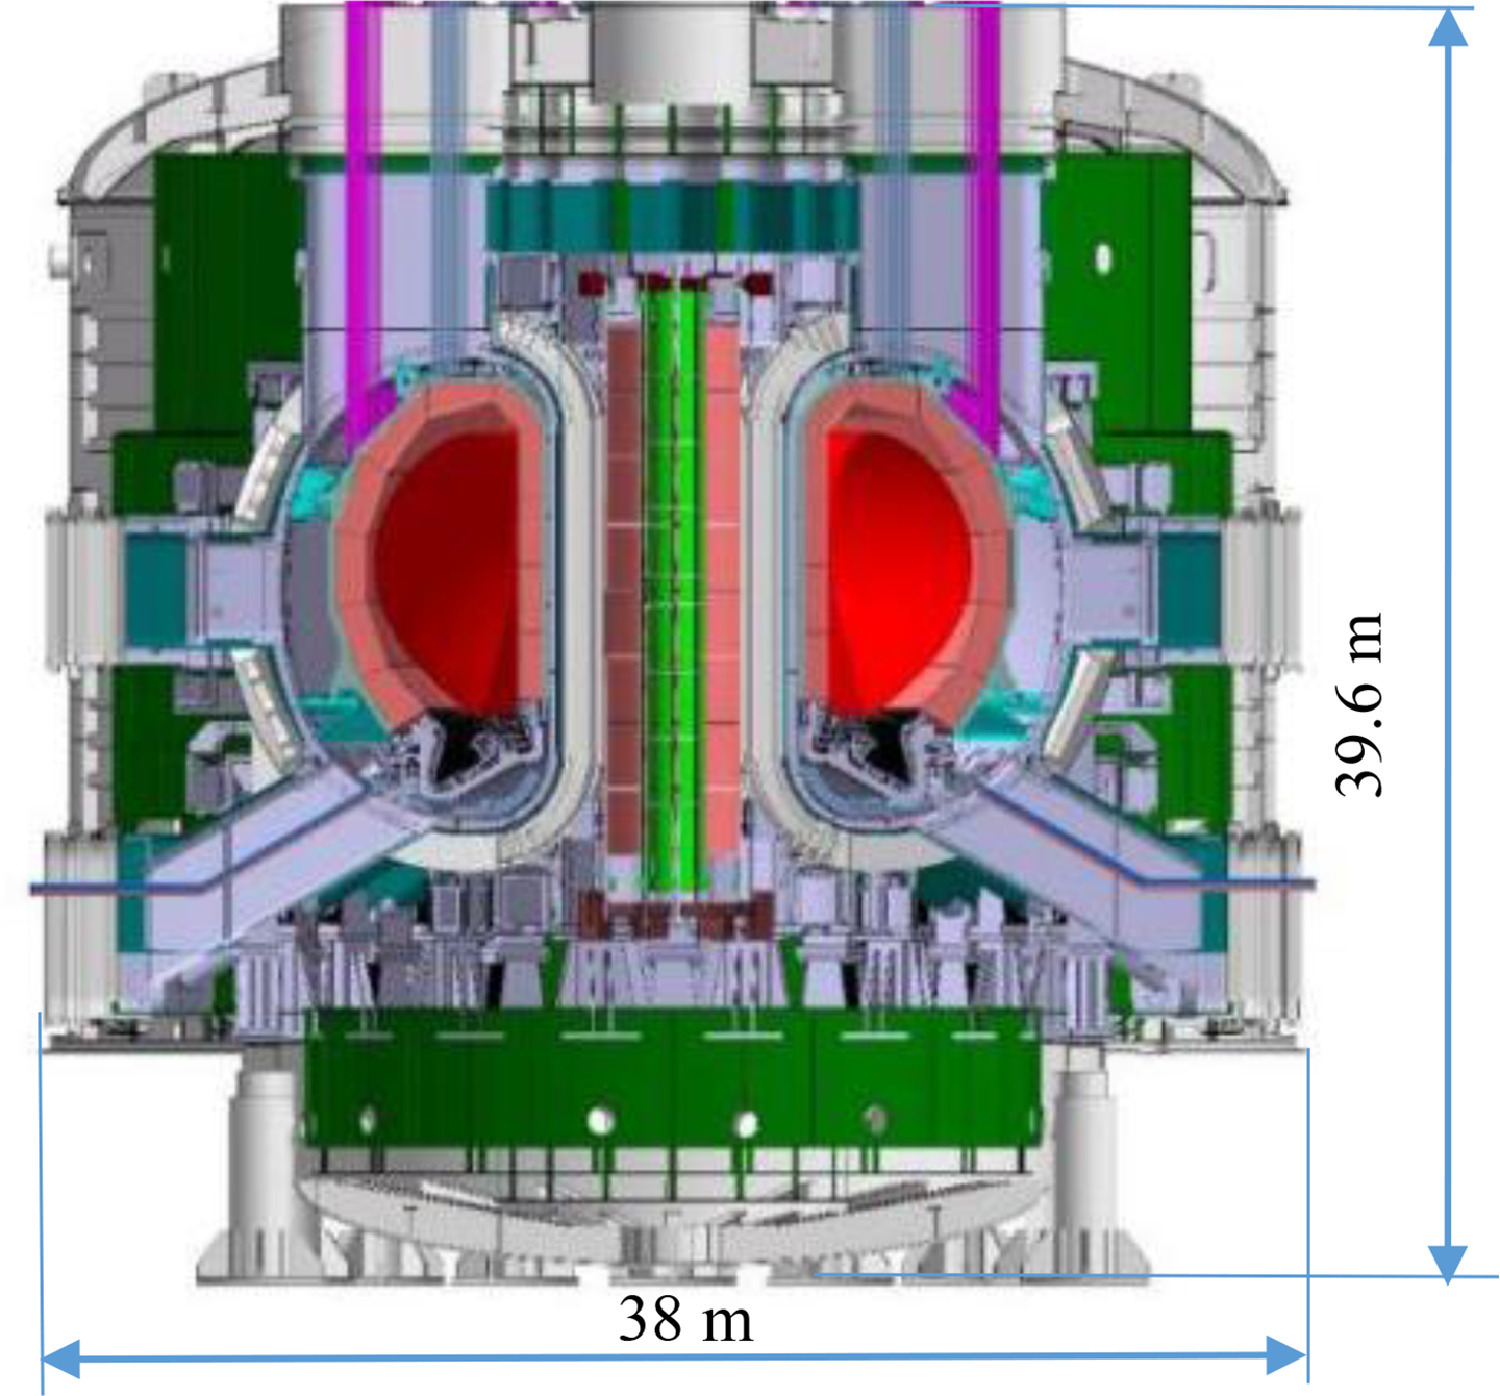
\includegraphics[width=0.5\textwidth]{files/CFETR_tokamak.jpg}
\caption{Configuration of the CFETR tokamak machine \parencite{CFETRCONFIG2022}.}
\label{fig:CFETR}
\end{figure}

\subsection{Selected activities' introduction}

\vskip 10pt

\begin{center}
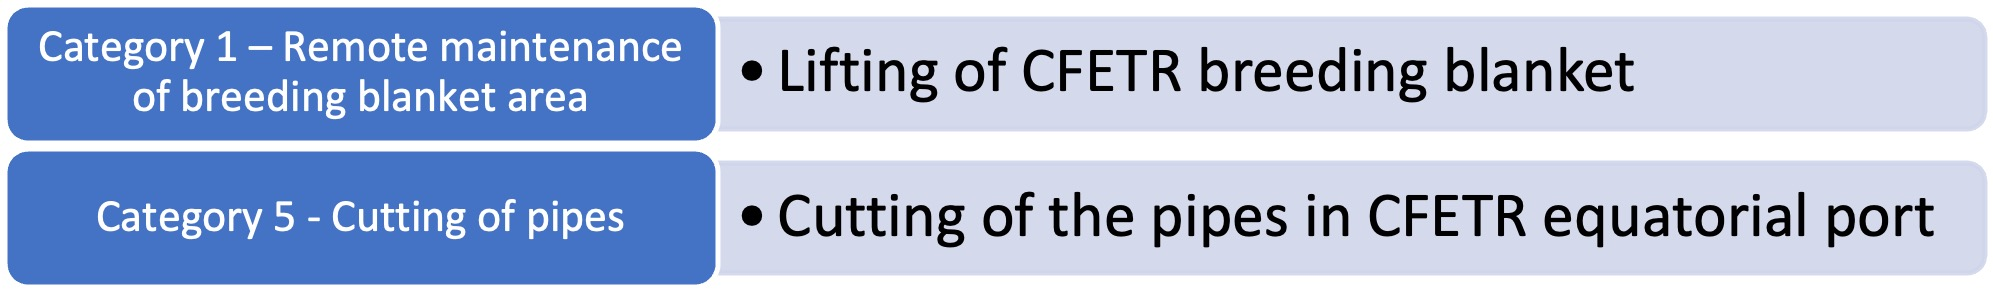
\includegraphics[width=15.24cm]{files/Activities.jpg}
\end{center}

\newpage

\subsubsection{Lifting of CFETR breeding blanket}

Three candidate tritium breeding blanket (TBB) concepts are proposed for CFETR; the solid blanket, i.e. helium cooled ceramic breeder (HCCB) blanket, water cooled ceramic breeder (WCCB) blanket, and the liquid blanket as supercritical CO\textsubscript{2} cooled lithium-lead (COOL) blanket \parencite{TBBCONFIG}.

For this report we will be focussing on the HCCB TBB as shown in \cref{fig:combined_blanket}.

\begin{figure}[htbp]
\centering
    \begin{subfigure}{0.48\textwidth}  % Using slightly less than 0.5 to allow for margins
        \centering
        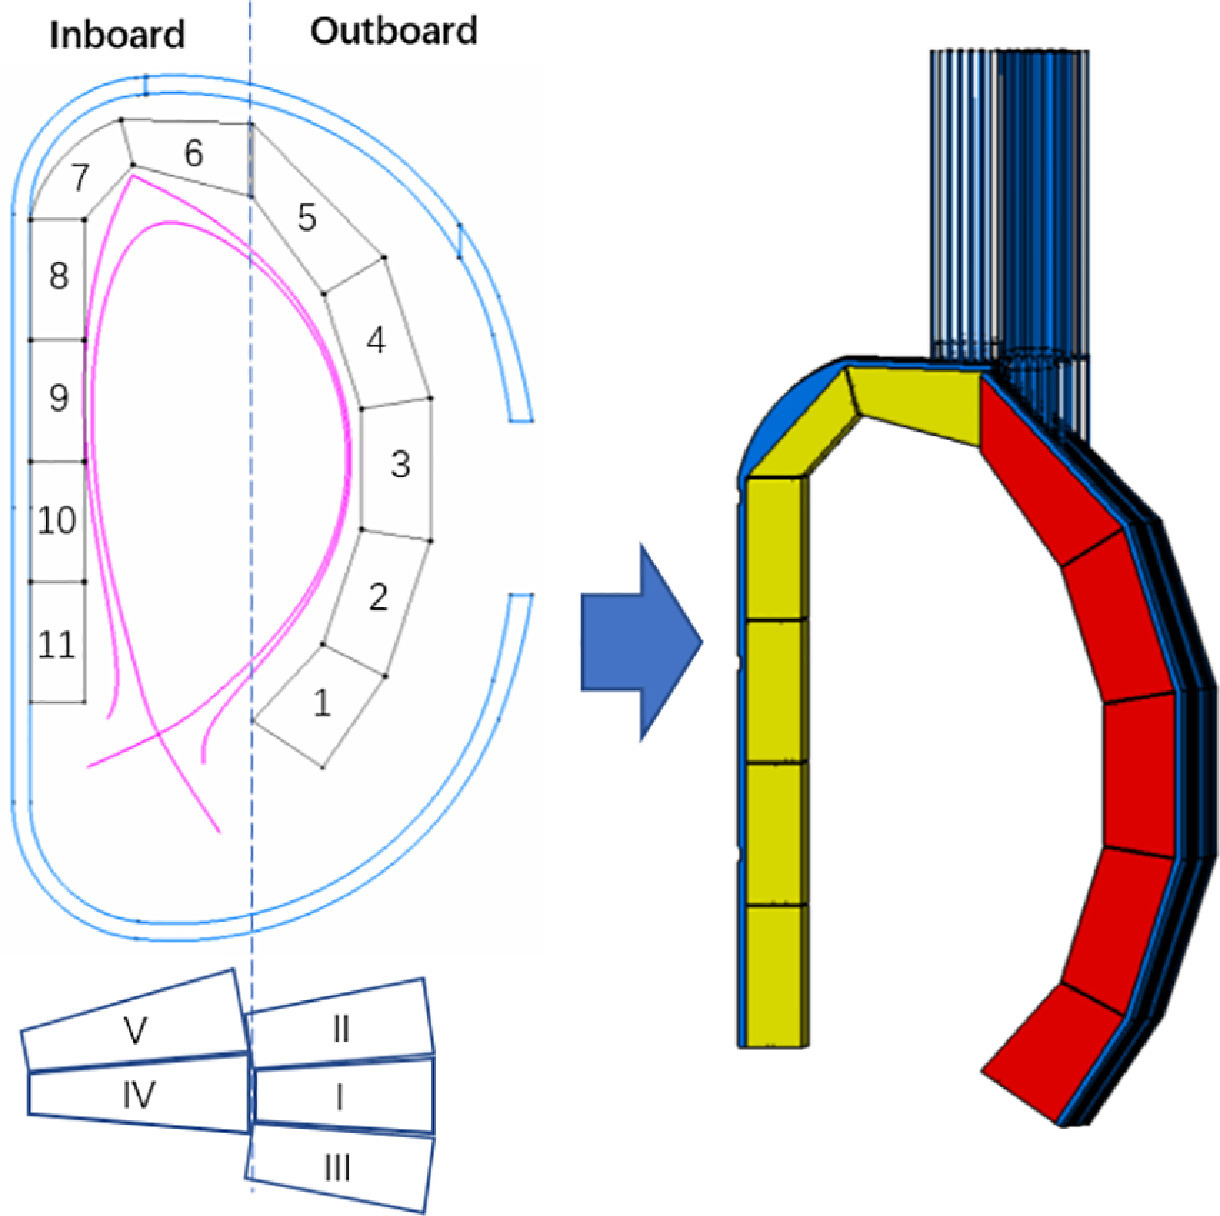
\includegraphics[width=\textwidth]{files/TBBCONFIG.jpg}
        \caption{Layout configuration of CFETR TBB.}
        \label{fig:HCCB}
    \end{subfigure}
    \hfill % This pushes the two images to the far left and far right
    \begin{subfigure}{0.48\textwidth}
        \centering
        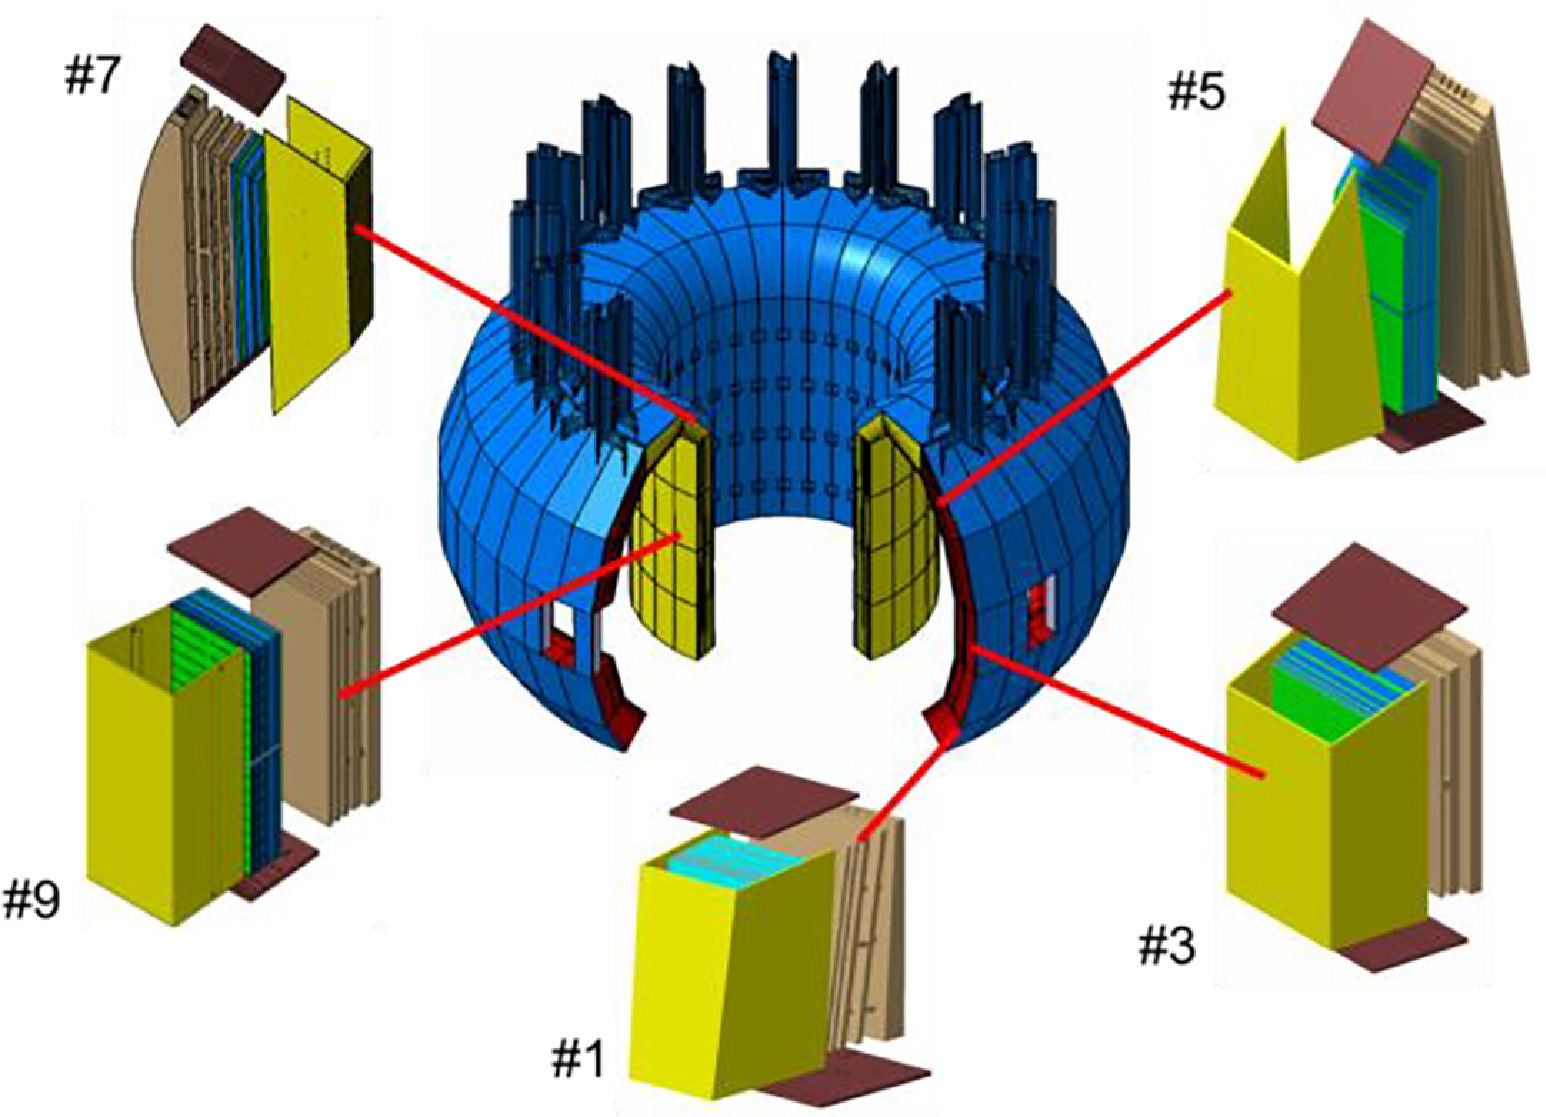
\includegraphics[width=\textwidth]{files/HCCBTBBmodules.jpg}
        \caption{Blanket modules design of HCCB TBB.}
        \label{fig:BB_lift}
    \end{subfigure}
    \vskip 10pt
    \caption{Overview of the HCCB TBB breeding blanket configuration and blanket modules design \parencite{HCCBTBB}.}
    \label{fig:combined_blanket}
\end{figure}

\vskip 10pt

The HCCB TBB architecture comprises 16 sectors. The sectors are further divided into two inboard and three outboard segments, each containing various specialized modules numbered 1 to 11 \parencite{TBBCONFIG}. 

\vskip 10pt

\begin{table}[htbp]
    \caption{Key parameters of the HCCB TBB \parencite{CFETRCONFIG2022}.}
    \begin{tabular}{|p{0.5\textwidth}|p{0.5\textwidth}|}
        \hline
        \textbf{Parameter} & \textbf{Value} \\
        \hline
        \text{Structure material} & \text{Reduced Activation Ferritic Martensiti (RAFM)} \\
        \hline
        \text{Helium gas (coolant) pressure} & \text{8 MPa} \\
        \hline
        \text{Operating inlet/outlet temperature} & \text{300 °C/500 °C} \\
        \hline
        \text{Weight of each inboard segment} & \text{~50 tons} \\
        \hline
        \text{Weight of each outboard segment} & \text{~80 tons}\\
        \hline
        \text{Total weight} & \text{~5000 tons} \\
        \hline
    \end{tabular}
    \label{tab:TBB_parameters}
\end{table}

\newpage

The remote maintenance activity is carried out using the remote handling (RH) system. This system is composed of lifting, pedestal, and toroidal blanket transfer structures as shown in \cref{fig:RHS}, with independent control systems \parencite{RHTBB}.

\begin{figure}[htbp]
\centering
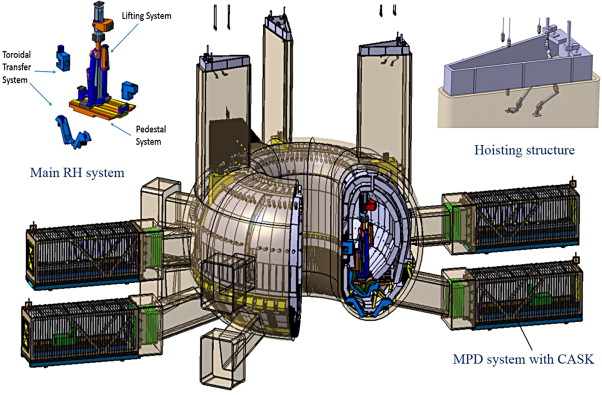
\includegraphics[width=0.5\textwidth]{files/RHTBB.jpg}
\caption{Remote handling system for the maintenance of HCBB TBB \parencite{RHTBB}.}
\label{fig:RHS}
\end{figure}

These systems are used to transport blanket segments, disassemble and install blanket supports, and hoist the blanket under the vertical ports during maintenance \parencite{CFETRCONFIG2022}.

\subsubsection{Cutting off the pipes in CFETR equatorial port}

The equatorial ports function as double-walled extensions of the vacuum vessel as shown in \cref{fig:EQPORT}.

\begin{figure}[htbp]
\centering
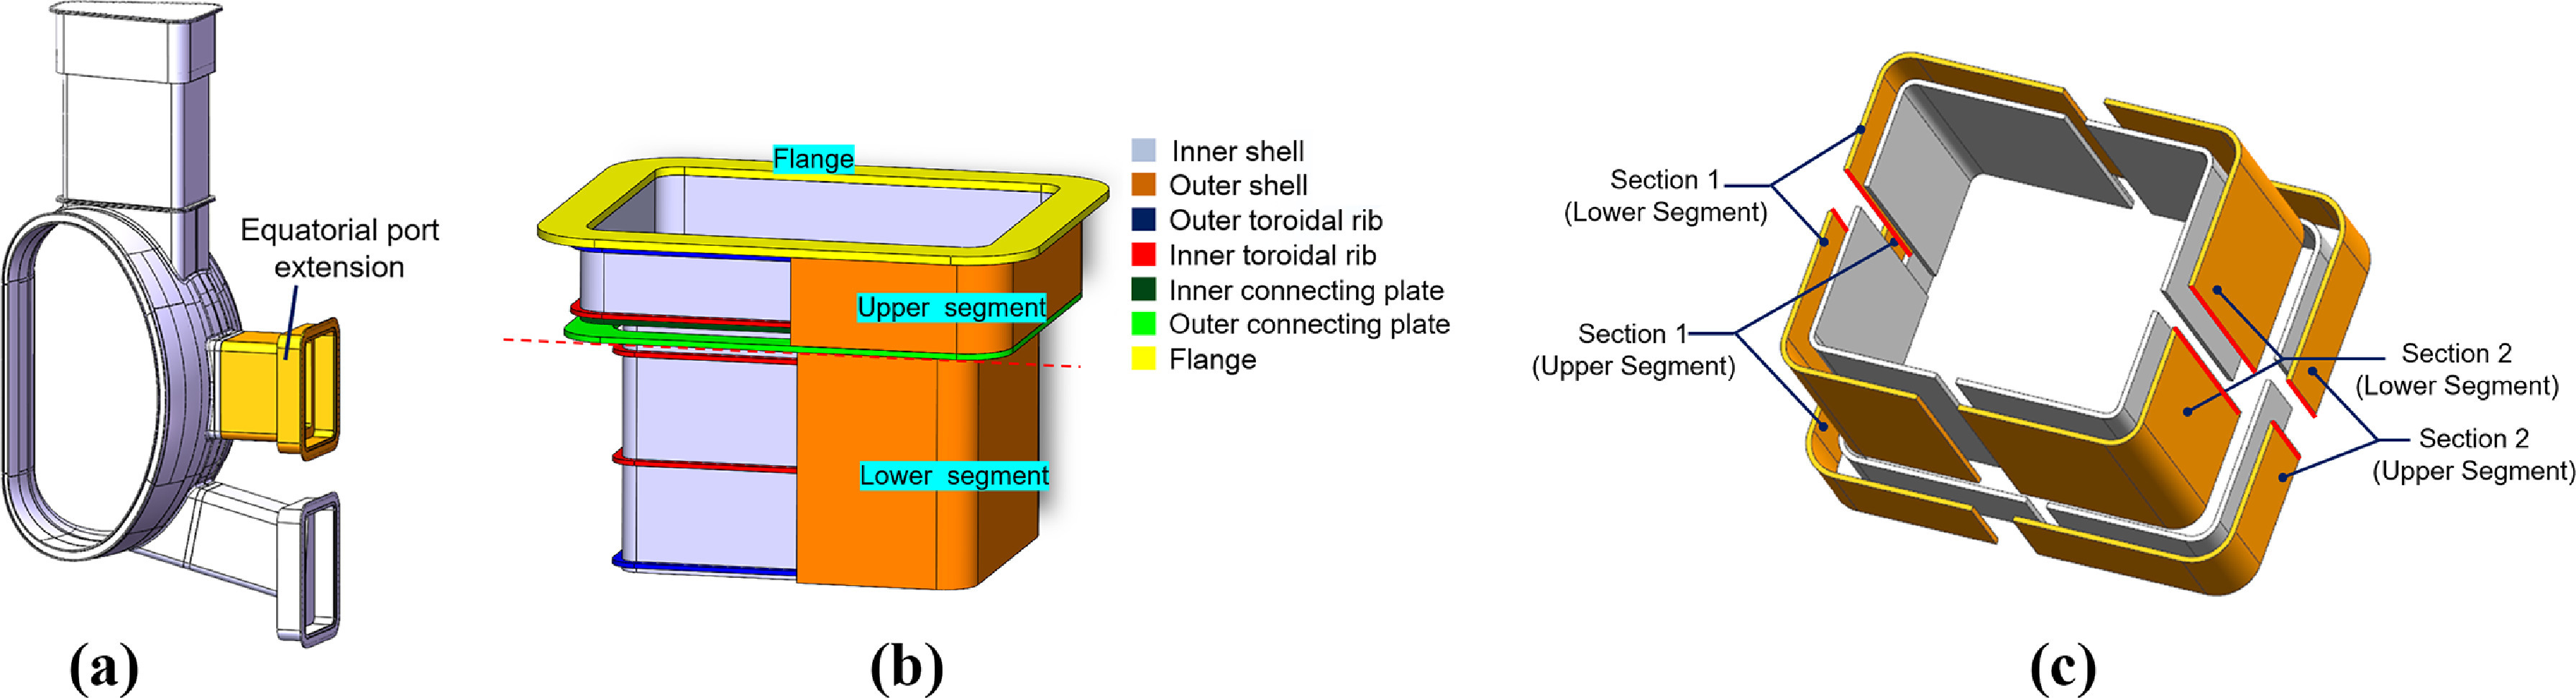
\includegraphics[width=\textwidth]{files/EQPORT.jpg}
\caption{Configuration of equatorial ports of CFETR \parencite{EQPORTCONFIG}.}
\label{fig:EQPORT}
\end{figure}

The vacuum vessel has 6 equatorial ports, 4 of which are used for maintenance and diagnostics, while the remaining 2 are for neutral beam injector (NBI) \parencite{CFETRCONFIG2022}.

\newpage

\begin{table}[htbp]
    \caption{Key parameters of the equatorial port \parencite{EQPORTCONFIG}.}
    \begin{tabular}{|p{0.5\textwidth}|p{0.5\textwidth}|}
        \hline
        \textbf{Parameter} & \textbf{Value} \\
        \hline
        \text{Length} & \text{4180 mm} \\
        \hline
        \text{Width} & \text{3620 mm} \\
        \hline
        \text{Height} & \text{2860 mm} \\
        \hline
        \text{Weight of each port} & \text{~90 tons}\\
        \hline
    \end{tabular}
    \label{tab:EQPORT_parameters}
\end{table}

The remote handling (RH) system used to maintain equatorial ports of the vacuum vessel include heavy duty manipulators located in horizontal casks. They are used to perform tasks like cutting and welding pipes \parencite{RHTBB}.

\begin{figure}[htbp]
\centering
\begin{subfigure}{0.48\textwidth}
    \centering
    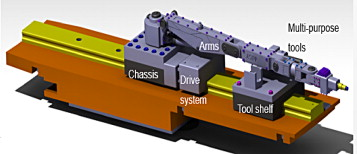
\includegraphics[width=\textwidth]{files/MPD.jpg}
    \caption{Multi-purpose deployer system (MPD) for the maintenance of equatorial port.}
    \label{fig:MPD}
\end{subfigure}
\begin{subfigure}{0.48\textwidth}
    \centering
    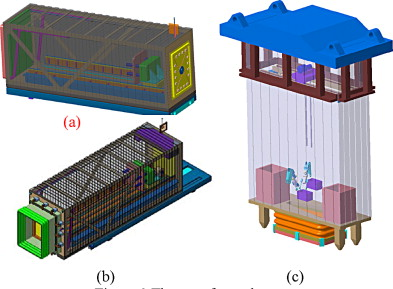
\includegraphics[width=\textwidth]{files/CASKs.jpg}
    \caption{Horizontal and vertical casks.}
    \label{fig:casks}
\end{subfigure}
\caption{Heavy duty manipulator and casks \parencite{RHTBB}.}
\label{fig:MPD_casks}
\end{figure}
\vskip 10pt
The CFETR is to have it's own dedicated MPD called the CMOR, CFETR multi-purpose overload robot.

\newpage
\section{Task 1}
This Task deals with creating a roadmap, the aim is to design one product capable of undertaking either of the remote maintenance activities described in the previous section. An implementation plan that matches the roadmap is also developed along with a bill of materials (EBOM).

\subsection{Roadmap}
The activity, lifting of CFETR breeding blanket was selected and a roadmap containing tasks from hiring the required personnel to the final delivery of the product is developed and visualized using a gantt chart.

\subsection{Implementation plan}
The tasks are divided among the team members and a detailed implementation plan is developed. The implementation plan includes the description of the task, the timeline for completion and a RACI matrix.

\subsection{Engineering bill of materials}
The machines for the remote maintenance of the HCCB TBB and cutting of pipes in the CFETR equatorial ports are listed in the chart below.
\vskip 10pt
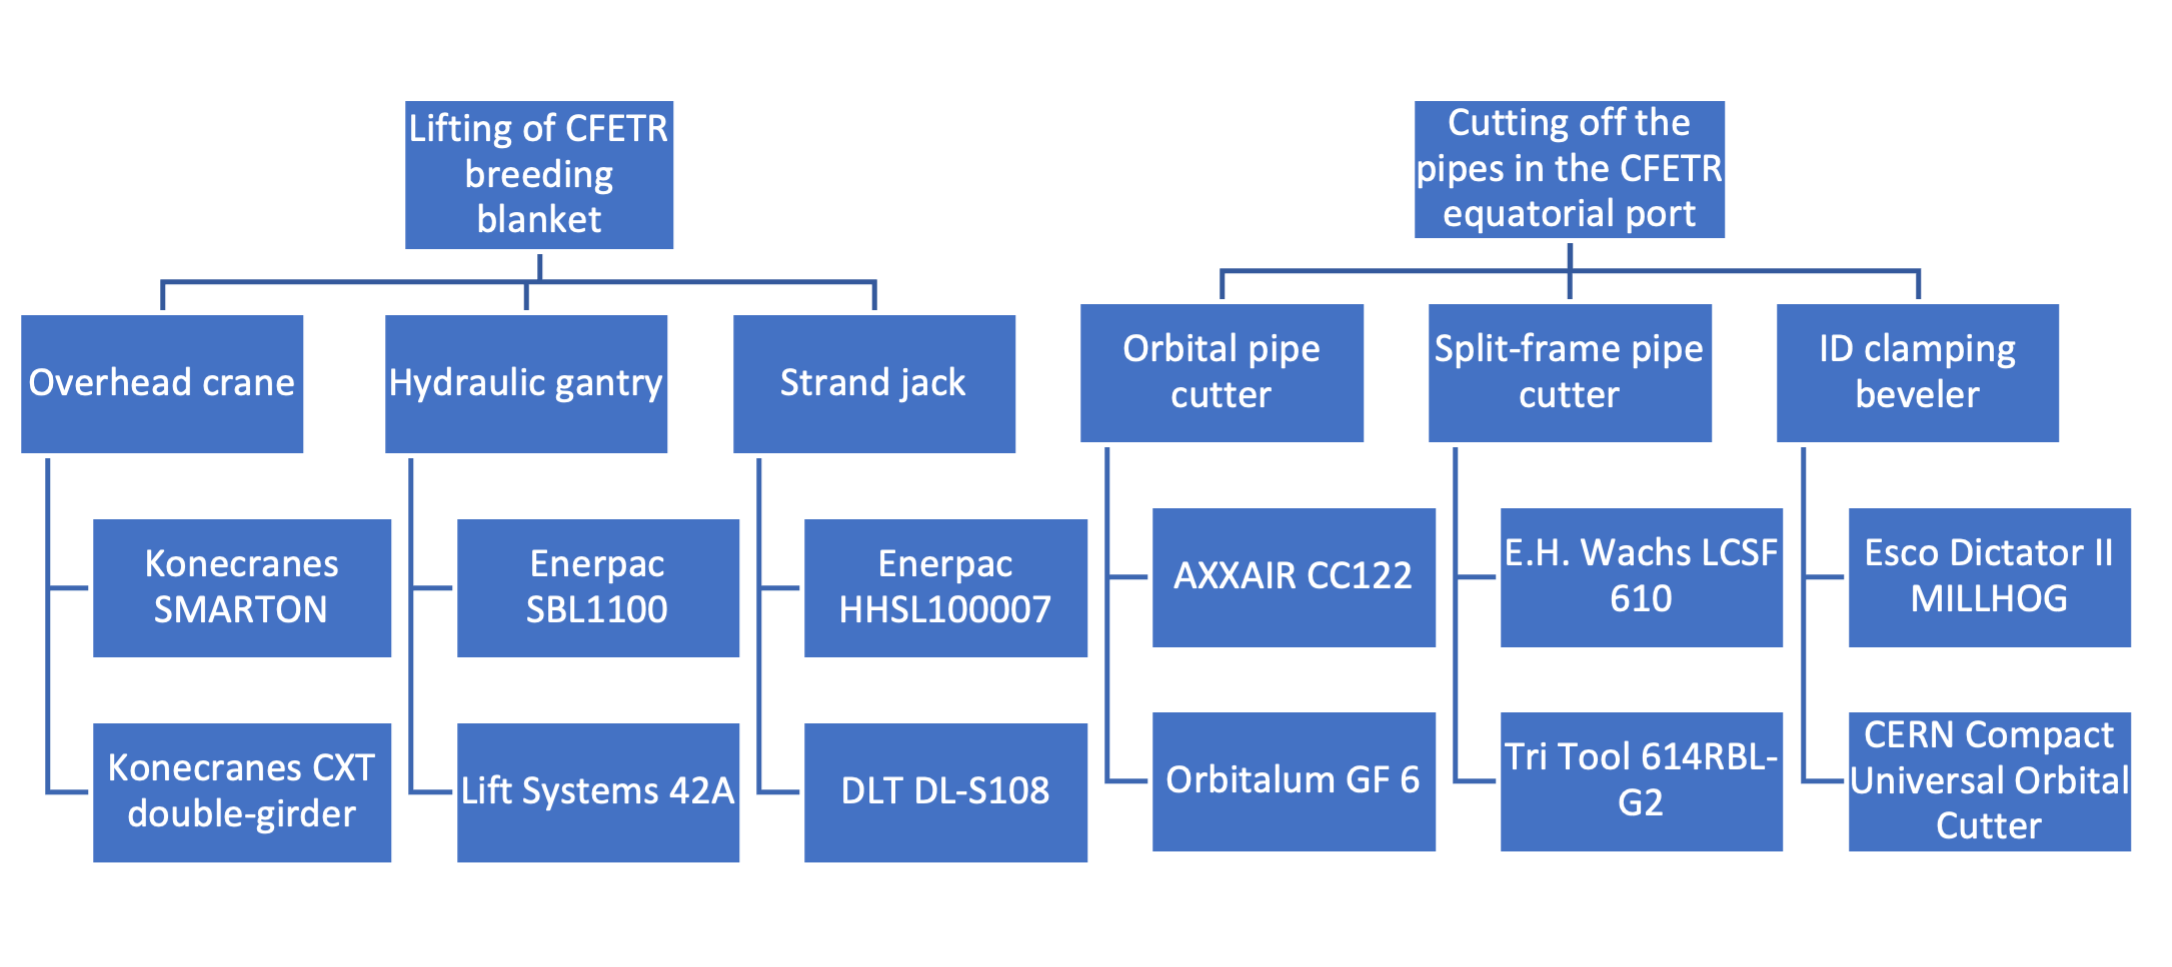
\includegraphics{files/EBOM.png}

\newpage
\section{Task 2}
Task 2 aims to document the literature review in a systematic way, including datasheet, system requirement document (SRD), and context definition document (CDD).

\subsection{Datasheet}
Workload was evenly distributed across the team, with each individual sourcing specific machines for the EBOM and subsequently completing the required datasheets for those same machines.

\subsection{System requirement document (SRD)}
While the EBOM was handled individually, the team worked together to build the System Requirements Document (SRD). Instead of splitting it up into separate parts, everyone collaborated on the whole thing. This allowed us to use everyone's expertise to create a more complete and accurate list of requirements.

\subsection{Context definition document (CDD)} 
The same was the case for the Context Definition Document (CDD). The team worked together to define the context of the project, ensuring that all aspects were considered and that the document was comprehensive.

\section{Conclusions}

The task was successfully completed, significantly enhancing our understanding of project planning and management. We gained thorough experience with core concepts such as the literature review, project roadmap, EBOM, and implementation plan. Ultimately, all project objectives were met in full.